\documentclass{article}

\usepackage[final]{neurips}
\usepackage[utf8]{inputenc} % allow utf-8 input
\usepackage[T1]{fontenc}    % use 8-bit T1 fonts
\usepackage{hyperref}  
\usepackage{amsmath}% hyperlinks
\usepackage{url} 

\usepackage{booktabs}       % professional-quality tables
\usepackage{amsfonts}       % blackboard math symbols
\usepackage{nicefrac}       % compact symbols for 1/2, etc.
\usepackage{microtype}      % microtypography
\usepackage{graphicx}
\usepackage{natbib}
\setcitestyle{numbers}

\usepackage{xepersian}
\settextfont{XB Yas.ttf}

\title{انتگرال}

\author{%
  نگین رحیمی یزدی\\
   نرم افزار ریاضی\\
  دانشگاه صنعتی امیرکبیر\\
  \texttt{neginrahimiyazdi@gmail.com} \\
}

\begin{document}


\begin{minipage}{0.1\textwidth}% adapt widths of minipages to your needs

\includegraphics[width=1.1cm]{Amirkabir.jpg}
\end{minipage}%
\hfill%
\begin{minipage}{0.9\textwidth}\raggedleft
دانشگاه امیرکبیر\\
\end{minipage}
% \end{}


\makepertitle


\section{مقدمه} 
در ریاضیات، انتگرال 
روشی برای اختصاص اعداد به توابع است، به گونه‌ای که جابجایی، مساحت، حجم و دیگر مفاهیم برآمده از ترکیب داده‌های بی‌نهایت کوچک را به وسیله آن بتوان توصیف کرد. انتگرال‌گیری یکی از دو عمل مهم در حساب دیفرانسیل و انتگرال است، که عمل دیگر آن (عمل معکوس) دیفرانسیل‌گیری یا همان مشتق‌گیری است.
\cite{Integral,Integralation,MultipleIntegral}

\section{انتگزال معین} 
انتگرال معین
\citep{Adams,Thomas}


$$\int_a^{b}x dx$$
\begin{figure}[!h]
    \centering
    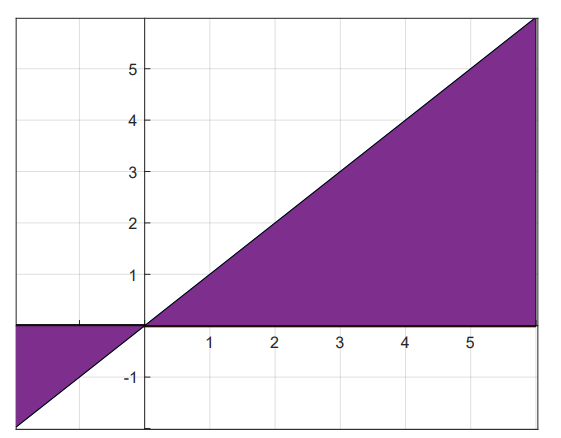
\includegraphics[width=6cm]{code2Integralpic.png}
    \caption{انتگرال $y=x$}
    \label{fig:انتگرال خط}
\end{figure}

\begin{figure}[!h]
    \centering
    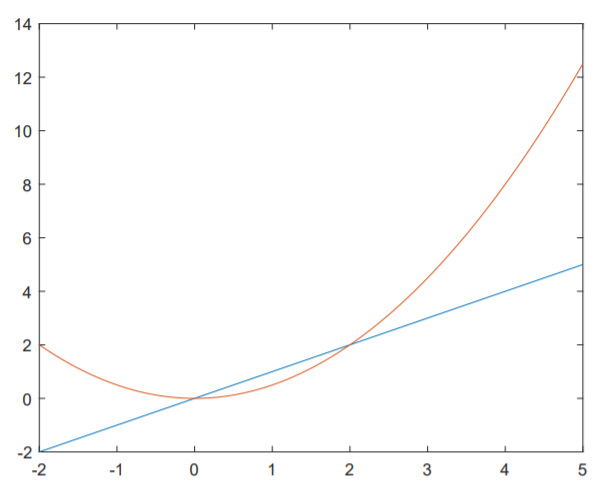
\includegraphics[width=6cm]{code1integral.png}
    \caption{انتگرال $y=x$}
    \label{fig:انتگرال خط}
\end{figure}

\begin{figure}[!h]
    \centering
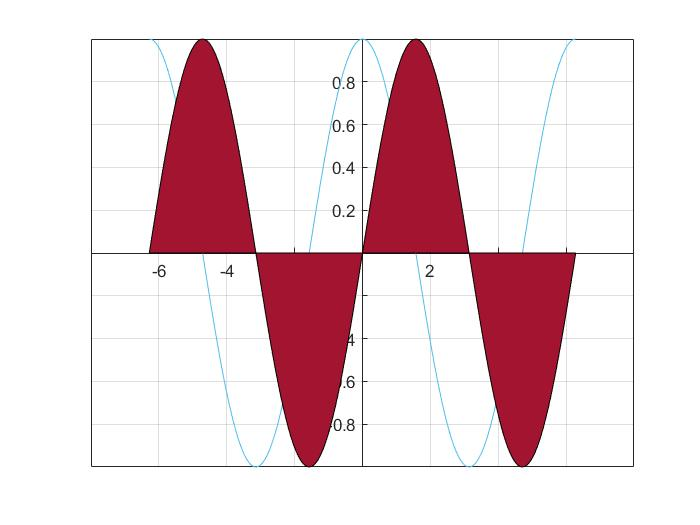
\includegraphics[width=7cm]{code3Integral3.jpg}
    \caption{انتگرال $y=sin(x)$}
    \label{fig:انتگرال خط}
\end{figure}


\begin{figure}[!h]
    \centering
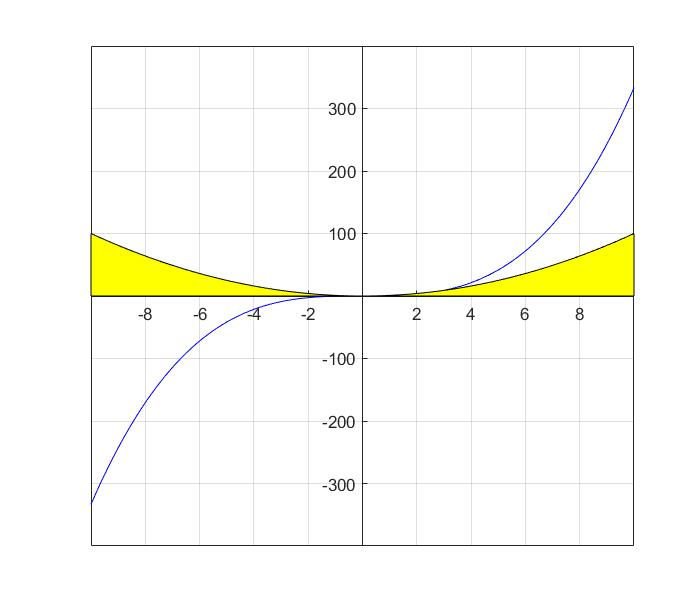
\includegraphics[width=6cm]{x2.jpg}
    \caption{انتگرال $y=x^2$}
    \label{fig:انتگرال خط}
\end{figure}
\newpage
\section{تقریب انتگرال‌های معین}
محاسبه سطح زیر نمودار به‌وسیله مستطیل‌هایی زیر نمودار. هر چه قدر عرض مستطیل‌ها کوچک می‌شوند مقدار دقیق تری از مقدار انتگرال بدست می‌آید.


انتگرال‌های معین ممکن است با استفاده از روش‌های انتگرال‌گیری عددی، تخمین زده شوند. یکی از عمومی‌ترین روش‌ها، روش مستطیلی نامیده می‌شود در این روش ناحیه زیر نمودار تابع به یک سری مستطیل تبدیل شده و جمع مساحت آن‌ها نشان دهنده مقدار تقریبی انتگرال است. از دیگر روش‌هایی معروف برای تخمین مقدار انتگرال روش سیمپسون و روش ذوزنقه‌ای است. اگر چه روش‌های عددی مقدار دقیق انتگرال را به ما نمی‌دهند ولی در بعضی از مواقع که انتگرال تابعی قابل حل نیست یا حل آن مشکل است کمک زیادی به ما می‌کند.\citep{Numerical}


\begin{figure}[!h]
    \centering
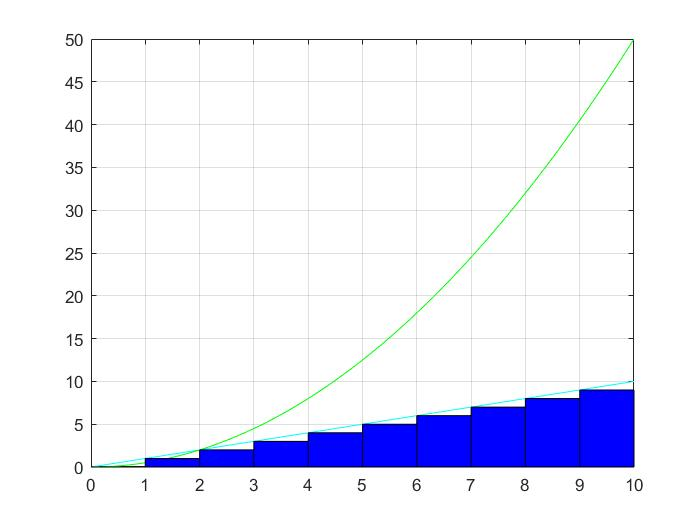
\includegraphics[width=7cm]{pic6integral.jpg}
    \caption{
    جمع پایینی داربوسک برای تابع 
    $y=x$
    }
    \label{fig:انتگرال خط}
\end{figure}


\begin{figure}[!h]
    \centering
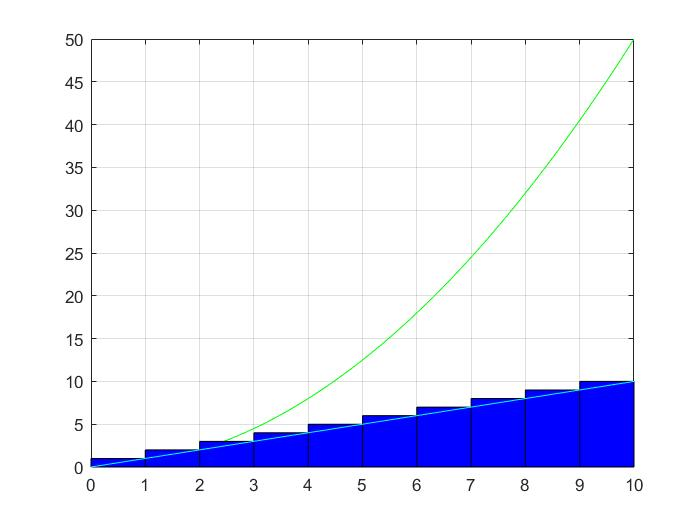
\includegraphics[width=7cm]{pic7integral.jpg}
    \caption{
    جمع بالایی داربوسک برای تابع 
    $y=x$
    }
    \label{fig:انتگرال خط}
\end{figure}

\begin{figure}[!h]
    \centering
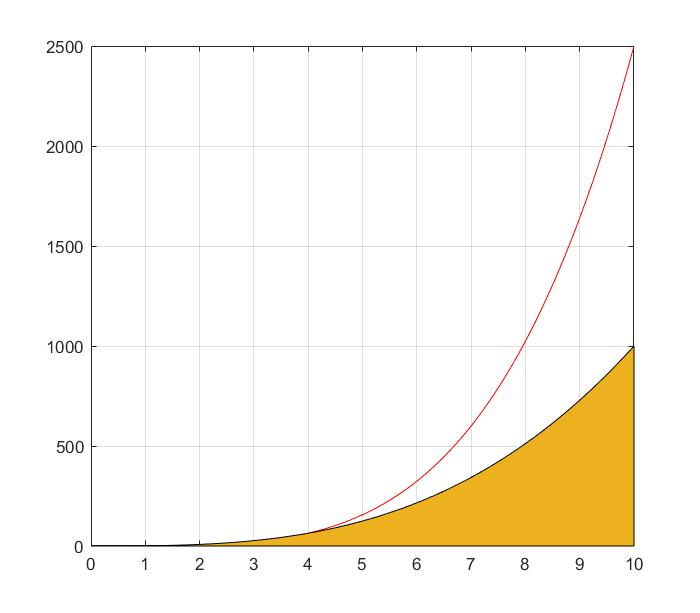
\includegraphics[width=7cm]{x33.jpg}
    \caption{انتگرال $y=x^3$}
    \label{fig:انتگرال خط}
\end{figure}

\begin{figure}[!h]
    \centering
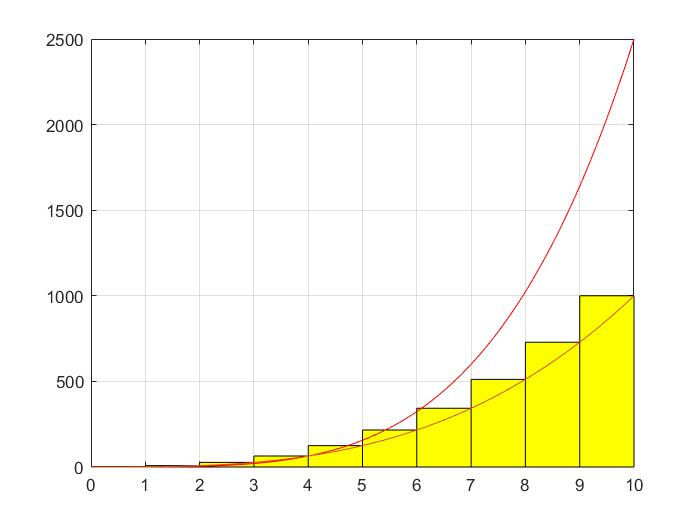
\includegraphics[width=7cm]{pic8integral.jpg}
    \caption{جمع بالایی داربوسک برای تابع $y=x^3$}
    \label{fig:انتگرال خط}
\end{figure}

\begin{figure}[!h]
    \centering
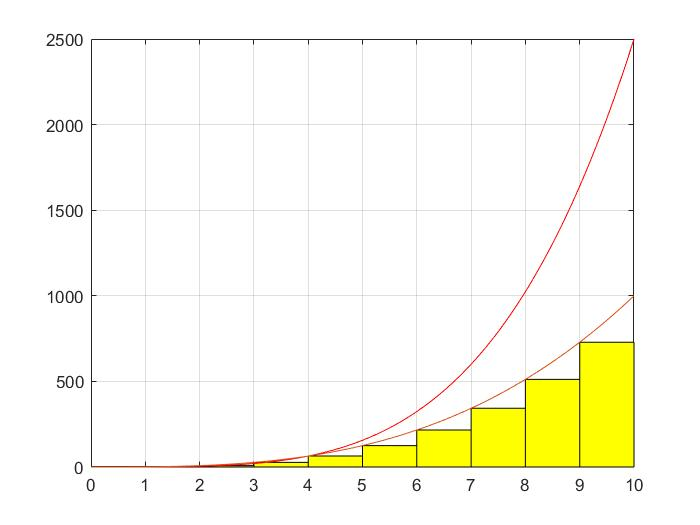
\includegraphics[width=7cm]{pic9code9Integal.jpg}
    \caption{جمع پایینی داربوسک برای تابع $y=x^3$}
    \label{fig:انتگرال خط}
\end{figure}
\newpage

\begin{figure}[!h]
    \centering
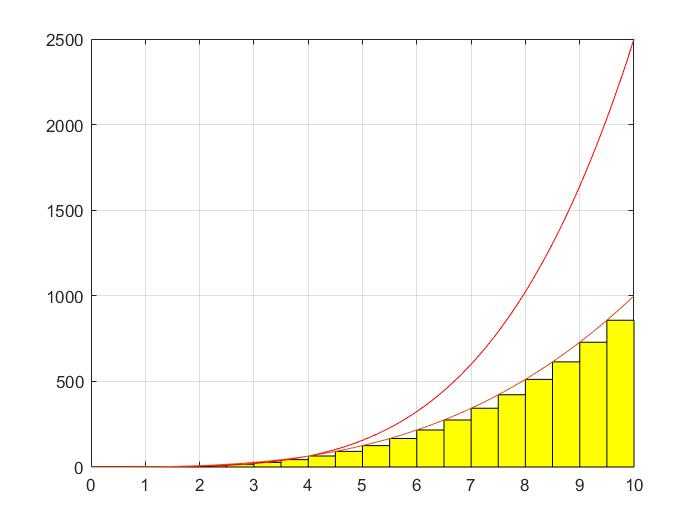
\includegraphics[width=7cm]{piccode10integral.jpg}
    \caption{جمع پایینی داربوسک برای تابع $y=x^3$}
    \label{fig:انتگرال خط}
\end{figure}

\begin{figure}[!h]
    \centering
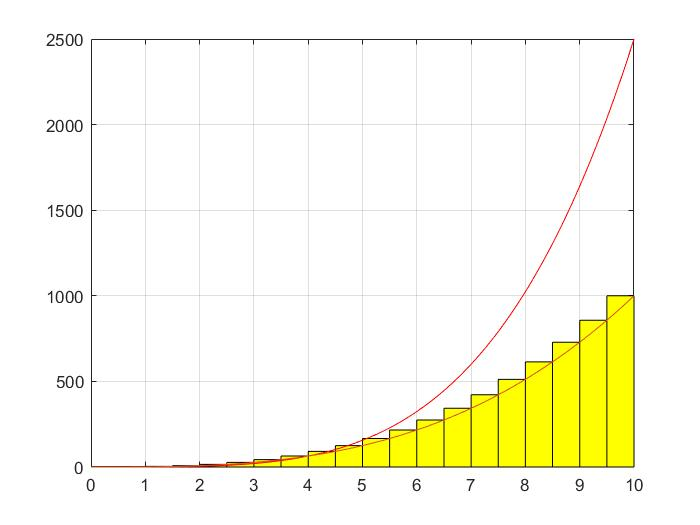
\includegraphics[width=8cm]{piccode11integral.jpg}
    \caption{جمع بالایی داربوسک برای تابع $y=x^3$}
    \label{fig:انتگرال خط}
\end{figure}

\begin{figure}[!h]
    \centering
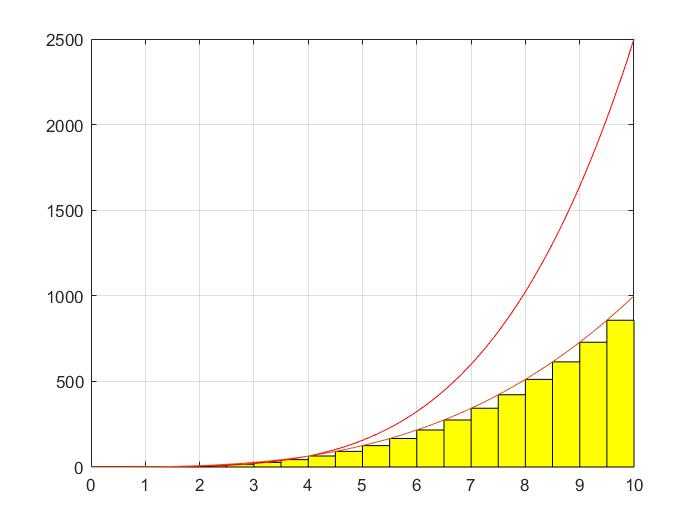
\includegraphics[width=8cm]{pic12codeIntegral.jpg}
    \caption{جمع پایینی داربوسک برای تابع $y=x^3$}
    \label{fig:انتگرال خط}
\end{figure}

\begin{figure}[!h]
    \centering
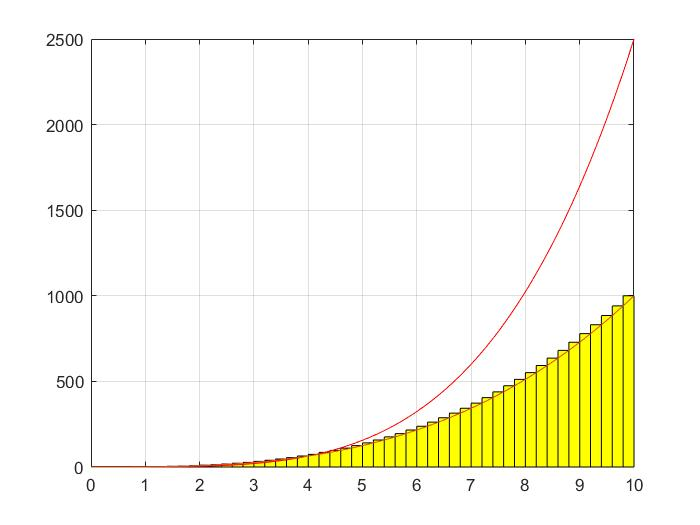
\includegraphics[width=8cm]{pic14codeIntegral.jpg}
    \caption{جمع بالایی داربوسک برای تابع $y=x^3$}
    \label{fig:انتگرال خط}
\end{figure}

\begin{figure}[!h]
    \centering
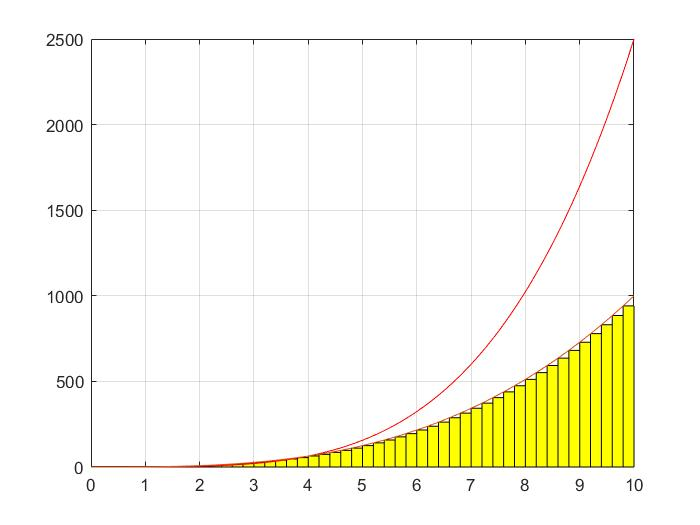
\includegraphics[width=8.2cm]{pic13codeIntegral.jpg}
    \caption{جمع پایینی داربوسک برای تابع $y=x^3$}
    \label{fig:انتگرال خط}
\end{figure}

\begin{figure}[!h]
    \centering
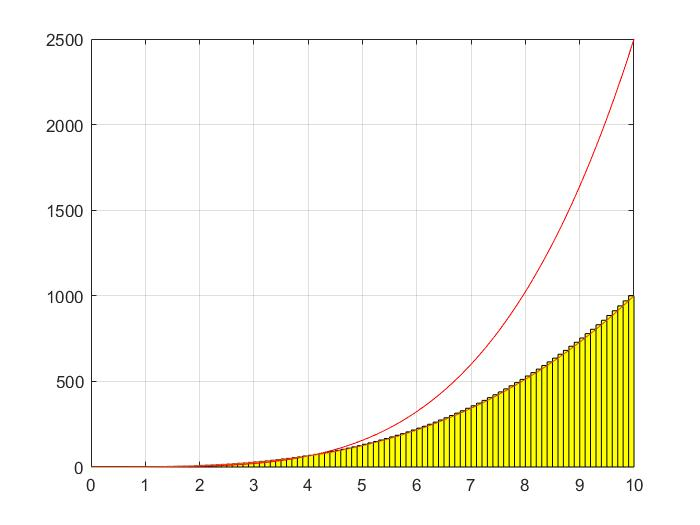
\includegraphics[width=8.2cm]{pic15codeIntegral.jpg}
    \caption{جمع بالایی داربوسک برای تابع $y=x^3$}
    \label{fig:انتگرال خط}
\end{figure}

\begin{figure}[!h]
    \centering
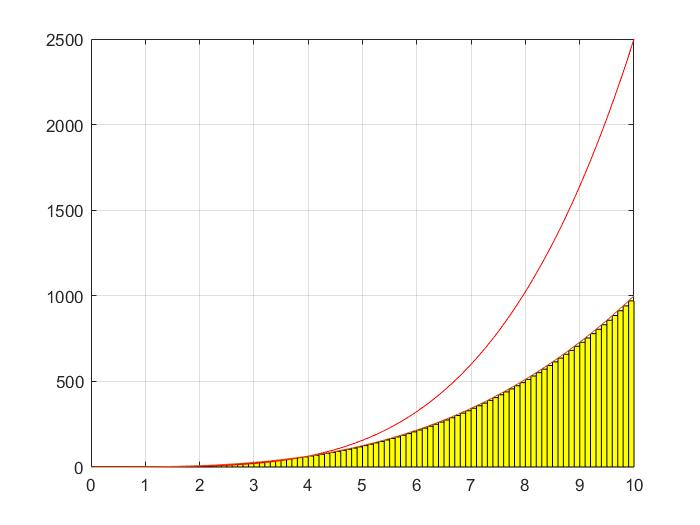
\includegraphics[width=8.2cm]{pic16codeIntegral.jpg}
    \caption{جمع پایینی داربوسک برای تابع $y=x^3$}
    \label{fig:انتگرال خط}
\end{figure}

\pagebreak

\begin{figure}[!h]
    \centering
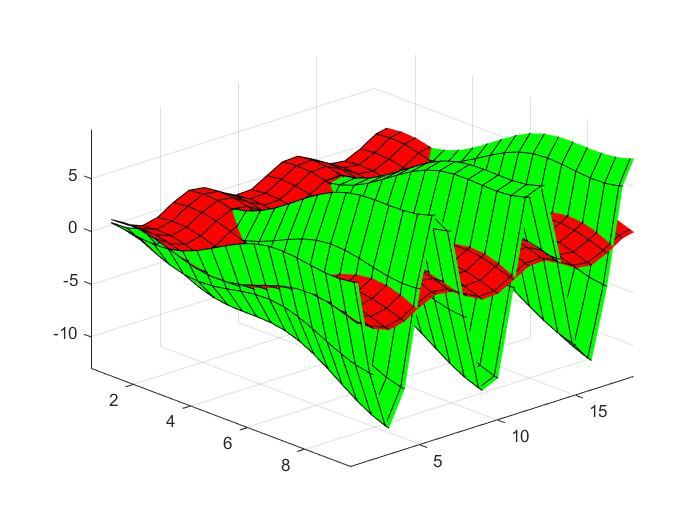
\includegraphics[width=8.2cm]{pic17codeIntegral.jpg}
    \caption{تابع انتگرال $z=cos(x)+sin(y)$ نسبت به  $x$}
    \label{fig:انتگرال خط}
\end{figure}


\begin{figure}[!h]
    \centering
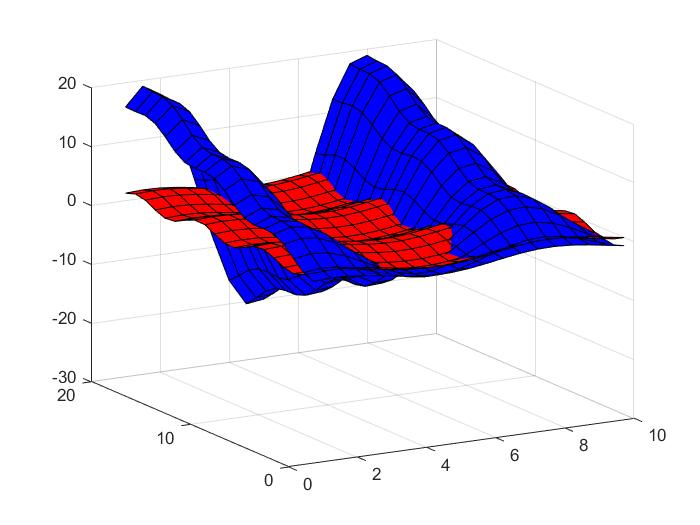
\includegraphics[width=8.2cm]{pic18codeIntegral.jpg}
  \caption{تابع انتگزال $z=cos(x)+sin(y)$نسبت به $y$}
    \label{fig:انتگرال خط}
\end{figure}

\begin{figure}[!h]
    \centering
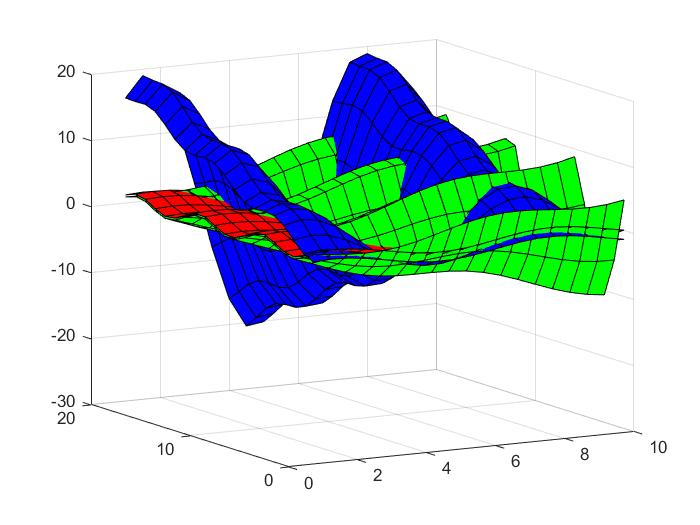
\includegraphics[width=8.2cm]{pic19codeIntegral.jpg}
 \caption{تابع انتگرال $z=cos(x)+sin(y)$ يکبار نسبت به $x$ يکبار نيسبت به $y$}
    \label{fig:انتگرال خط}
\end{figure}

\begin{figure}[!ht]
    \centering
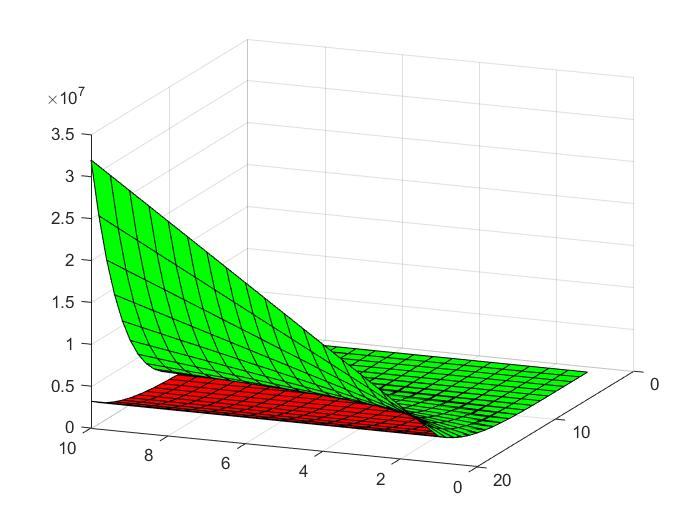
\includegraphics[width=7cm]{pic20codeIntegral.jpg}
    \caption{تابع انتگرال $z=x^2+y^5$ نسبت به $x$}
    \label{fig:انتگرال خط}
\end{figure}

\begin{figure}[!h]
    \centering
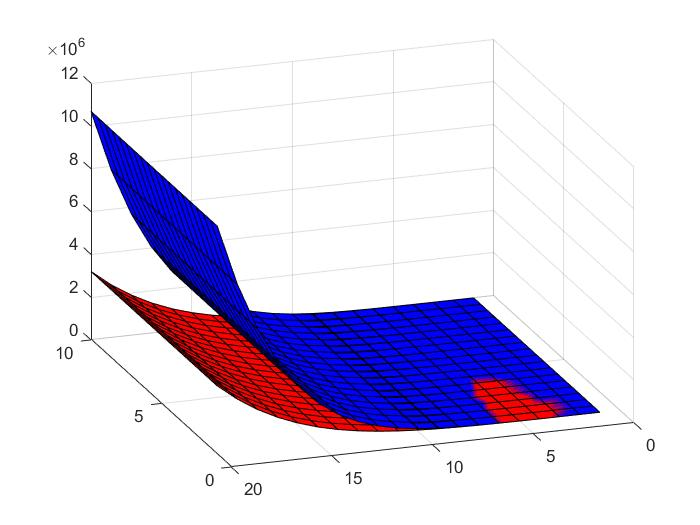
\includegraphics[width=7cm]{pic21codeIntegral.jpg}
 \caption{  تابع انتگرال $z=x^2+y^5$ نسبت به $y$}
    \label{fig:انتگرال خط}
\end{figure}


\begin{figure}[!h]
    \centering
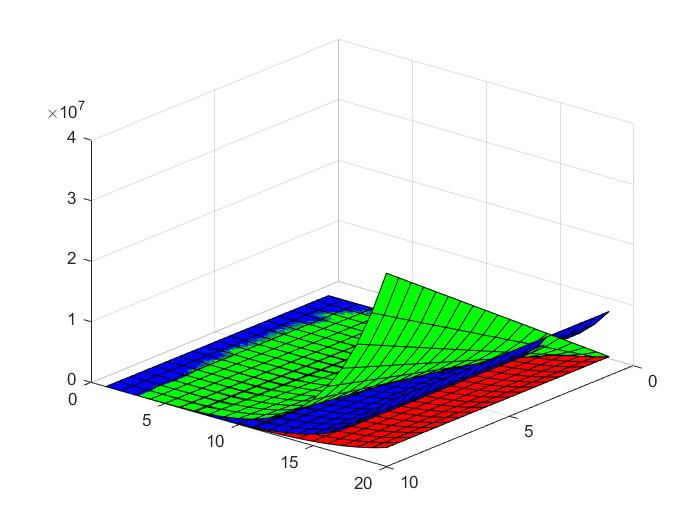
\includegraphics[width=7cm]{pic22codeIntegral.jpg}
    \caption{  تاپع انتگرال  $z=x^2+y^5$ نسبت به يکبار $y$ يکبار نسبت به $x$  }
    \label{fig:انتگرال خط}
\end{figure}

\begin{figure}[!h]
    \centering
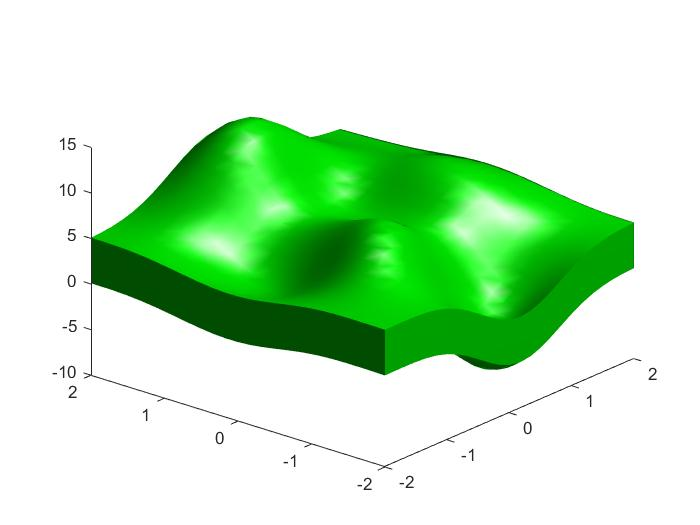
\includegraphics[width=9cm]{pic45Integral.jpg}
    \caption{    }
    \label{fig:انتگرال خط}
\end{figure}


\pagebreak

\section{ انتگرال گیری عددی}
در این بخش قصد داریم تقریبی برای 
$\int_a^{b} f(x)dx$
بیابیم.
انتگرال گیری عدی زمانی کاربرد دارد که نتوانیم به طور صریح و دقیق انتگرال مورد نظر را محاسبه کنیم.همچنین ممکن است به ضابطه تابع دسترسی نداشته باشیم و تنها مقادیر آن را در متناهی نقطه داشته باشیم .با استفاده از درون یابی اتگرال مورد نظر را با خطای محدود می یابیم.
\citep{Numerical_solution}
\section{قاعده نقطه میانی ساده}
تقریب انتگرال اینگونه به قضیه نقطه میانی ساده معروف است.
\citep{Numerical_solution}

\begin{align*}
    \int_a^{b} f(x)dx = \int_a^{b} p(x) dx  = \int_a^{b} f_{0}(x) dx = (b-a) f(\frac{a+b}{2}) =I_{0}(f)    
\end{align*}
        
\begin{figure}[!h]
    \centering
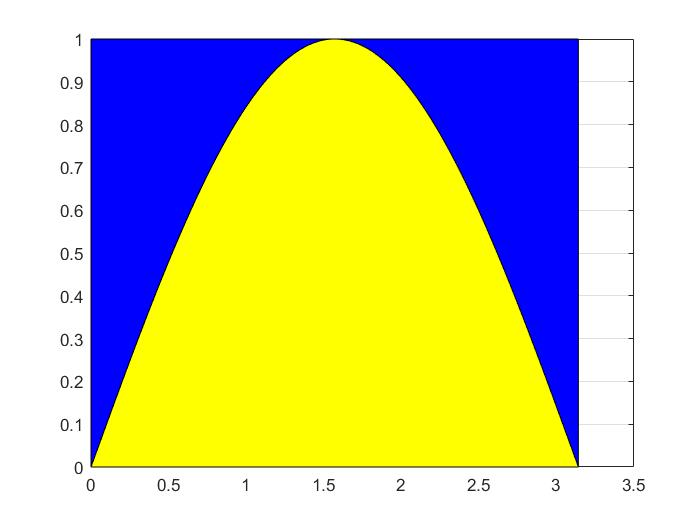
\includegraphics[width=9cm]{piccode24Integeral.jpg}
    \caption{  مقايسه مقدار انتگرال با انتگگرال گرفته شده در روش نقطه مياني $y=sin(x)$  }
    \label{fig:انتگرال خط}
\end{figure}

\begin{figure}[!h]
    \centering
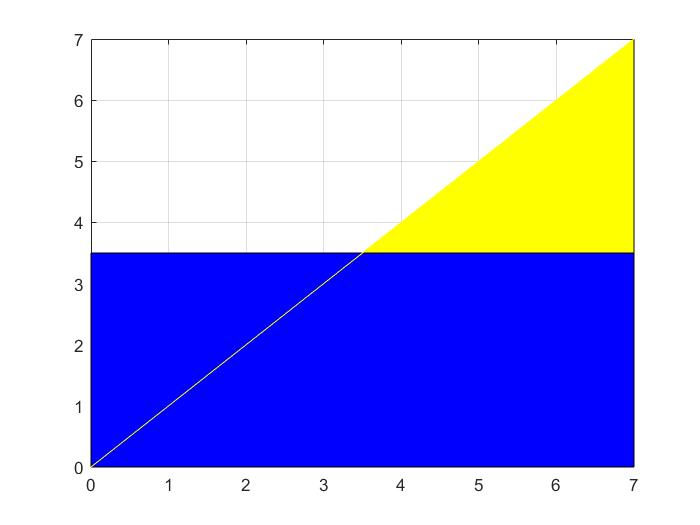
\includegraphics[width=9.5cm]{pic25codeIntegral.jpg}
    \caption{  مقايسه مقدار انتگرال با انتگرال گرفته شده در روش نقطه مياني $y=x$  }
    \label{fig:انتگرال خط}
\end{figure}

\begin{figure}[!h]
    \centering
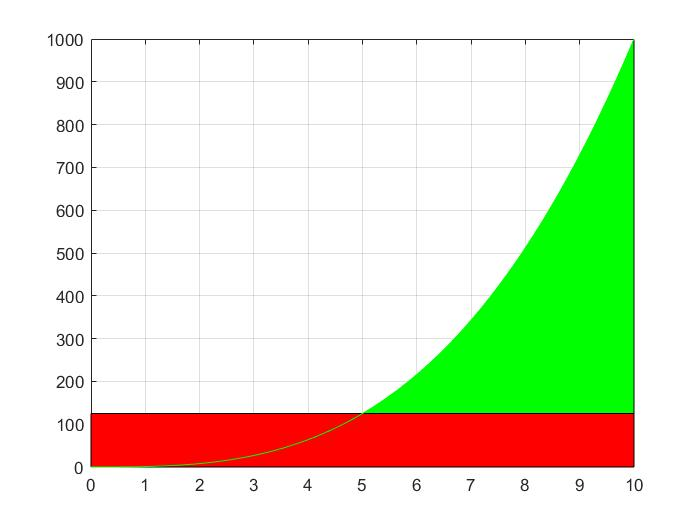
\includegraphics[width=9.5cm]{pic26codeIntegral.jpg}
    \caption{  مقايسه مقدار انتگرال با انتگرال گرفته شده در روش نقطه مياني $y=x^3$  }
    \label{fig:انتگرال خط}
\end{figure}

 ثابت می شود $c$
وجود دارد که خای اندازه گیری عددی نقطه میانی ساده برابر می شود با:
\\
\begin{align*}
    R_{0}(f) = \int_a^{b} f(x) dx - I_{0}(f) = (b-a)^3\frac{f''(c)}{24}
\end{align*}



\section{قاعده انتگرال گیری ذوزنقه ای ساده}
با استفاده از نقاط ابتدایی و انتهایی نمودار، 
نمودار را مانند ذوزنقه فرض می کنیم.
\\
\begin{align*}
    \int_{a}^b f(x) dx = \frac{b-a}{2}(f(a) + f(b)) = I_{1}(f)
\end{align*}


\begin{figure}[!h]
    \centering
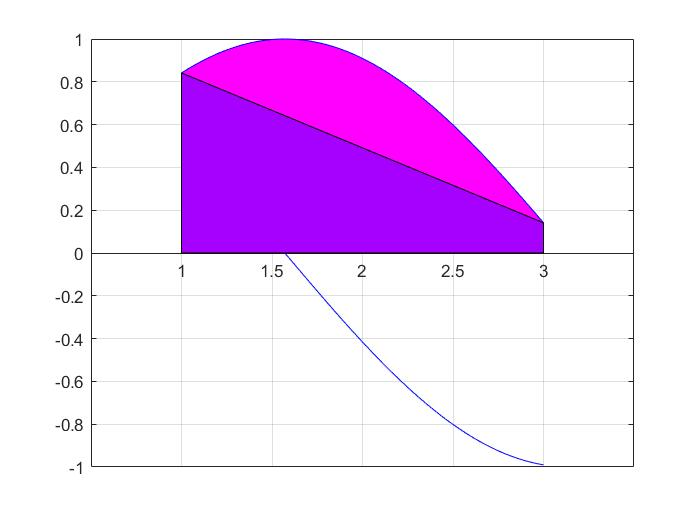
\includegraphics[width=9cm]{pic32codeIntegral.jpg}
    \caption{ روش ذوزنقه اي ساده $y=sin(x)$ }
    \label{fig:انتگرال خط}
\end{figure}

\begin{figure}[!h]
    \centering
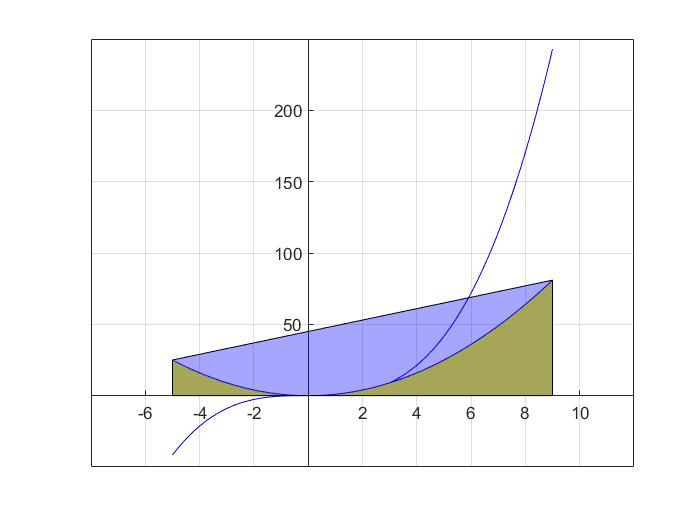
\includegraphics[width=9cm]{pic33codeIntegral.jpg}
    \caption{ روش ذوزنقه اي ساده $y=x^2$ }
    \label{fig:انتگرال خط}
\end{figure}


\begin{figure}[!h]
    \centering
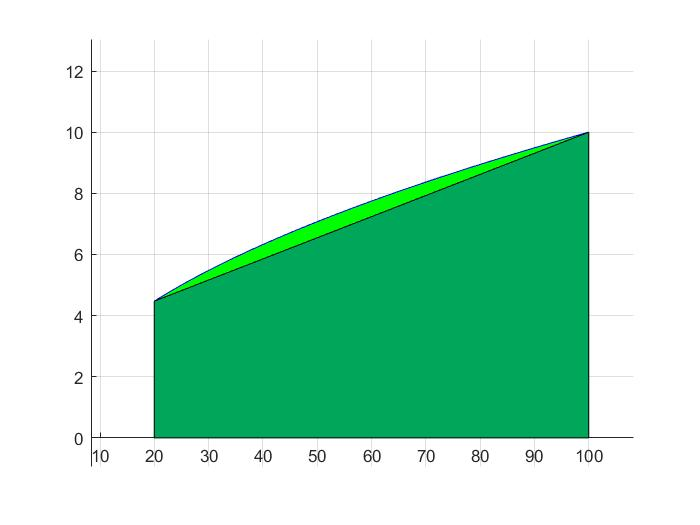
\includegraphics[width=7cm]{pic34codeIntegral.jpg}
    \caption{ روش ذوزنقه اي ساده $y=\sqrt x$ }
    \label{fig:انتگرال خط}
\end{figure}
 ثابت می شود $c$
وجود دارد که خطای اندازه گیری عددی ذوزنقه ای ساده برابر می شود با:
\\
\begin{align*}
    R_{1}(f) = \int_a^{b} f(x) dx - I_{1}(f) = -(b-a)^3\frac{f''(c)}{12}
\end{align*}


\section{درجه دقت فرمول های انتگرال های عددی}
درجه دقت یک فرمول انتگرال گیری عددی برابر $m$
است. هرگاه $m$
بزرگ ترین عدد صحیحی مثبتی باشد که فرمول مربوطه به توابع 
$f(x) = x^k$
که
$k=0,1,2,3,...$
دقیق است.
درجه دقت در روش ذوزنقعه ای و روش میانی برابر 1 است.
\citep{Numerical_integration}
\section{انتگرال گیری عددی مرکب}
به منظور کاهش خطا در تقریب 
$\int_a^{b} f(x) dx $
به ویزه زمانی که بازه انتگرال گیری بزرگ باشد،
ابتدا بازه را به زیر بازه هایی متساویی افاصله ننقسیم کرده و سپس 
از هر زیر بازه انتگرال می گیریم.
\citep{Numerical_integration}

\section{انتگرال گیری عددی نقطه میانی مرکب}
با در نظر گرفتن نقاط گسسته به صورت هم فاصله
انتگرال روی بازه $[a,b]$
را به انتگرال به زیر بازه ها تقسیم کرده و برای انتگرال رو ی هر زیر بازه از فرمول انتکرالگیری نقطه میانی استفاده می کنیم.پس داریم:


\begin{align*}
    M_{n}(f) = 2h \sum_{i=1}^{n/2} f(x_{2i-1})
\end{align*}



\begin{figure}[!h]
    \centering
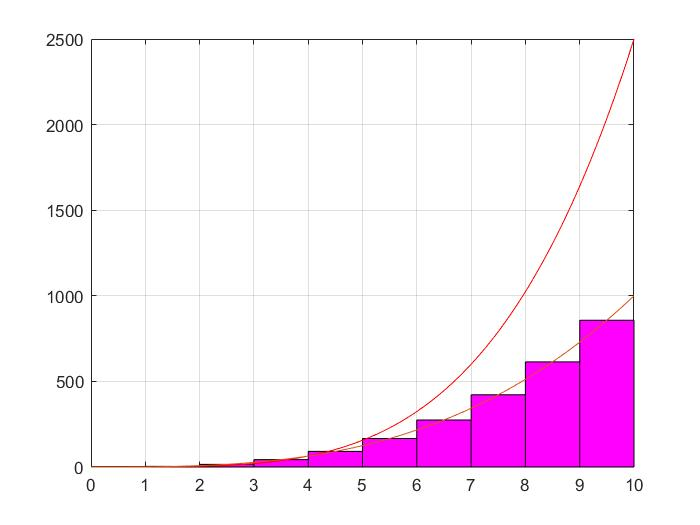
\includegraphics[width=7.5cm]{pic35codeIntegral.jpg}
    \caption{ روش نقطه میانی مرکب $y=x^3$ }
    \label{fig:انتگرال خط}
\end{figure}



\begin{figure}[!h]
    \centering
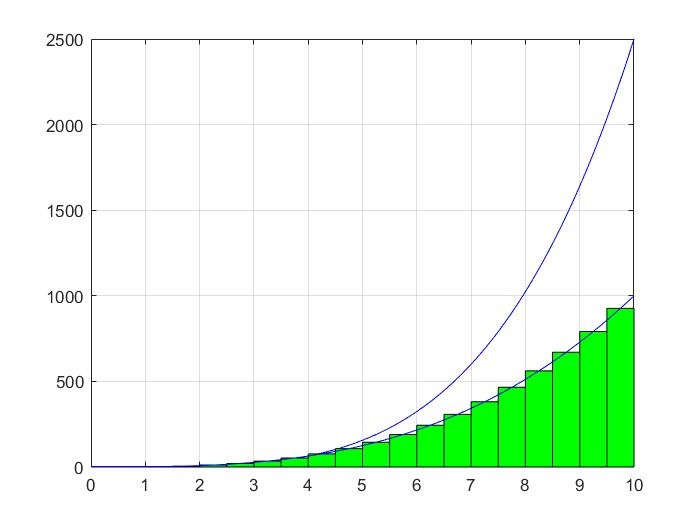
\includegraphics[width=8cm]{pic36codeIntegral.jpg}
    \caption{ روش نقطه میانی مرکب $y=x^3$ }
    \label{fig:انتگرال خط}
\end{figure}


\begin{figure}[!h]
    \centering
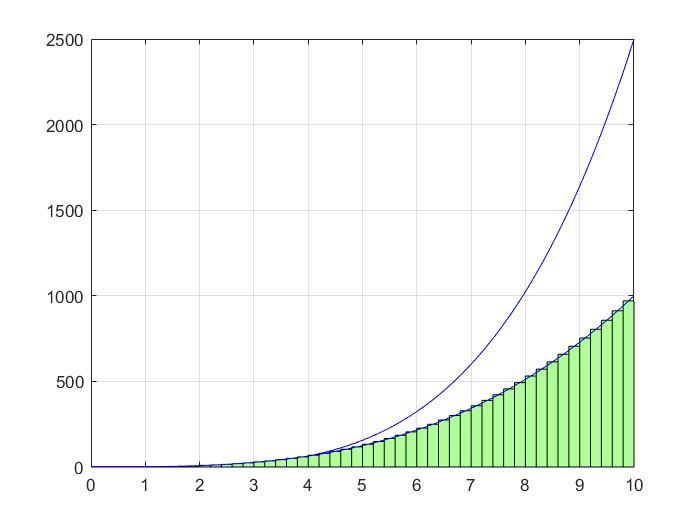
\includegraphics[width=8.4cm]{pic37codeIntegral.jpg}
    \caption{ روش نقطه میانی مرکب $y=x^3$ }
    \label{fig:انتگرال خط}
\end{figure}

\begin{figure}[!h]
    \centering
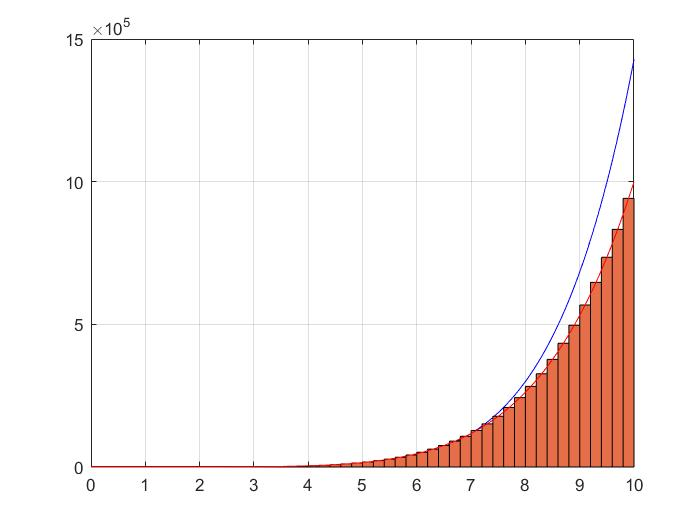
\includegraphics[width=8.4cm]{pic40codeintegral.jpg}
    \caption{ روش نقطه میانی مرکب $y=x^6$ }
    \label{fig:انتگرال خط}
\end{figure}

\begin{figure}[!h]
    \centering
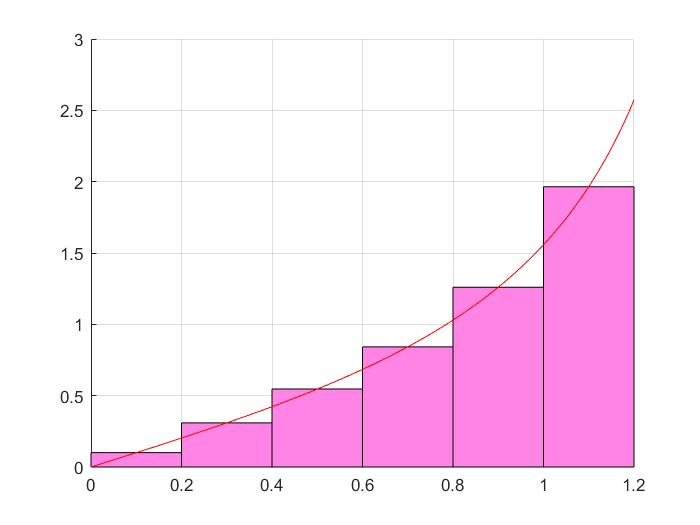
\includegraphics[width=8.2cm]{pic41codeIntegral.jpg}
    \caption{ روش نقطه میانی مرکب $y=tan(x)$ }
    \label{fig:انتگرال خط}
\end{figure}


\begin{figure}[!h]
    \centering
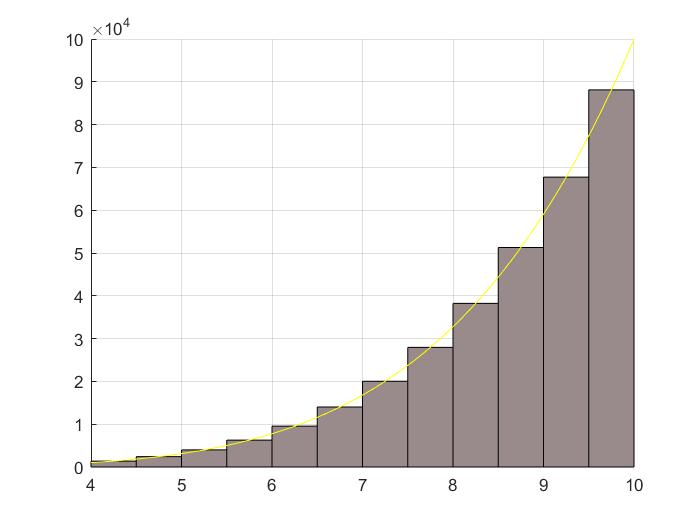
\includegraphics[width=8.2cm]{pic43IntegralCode.jpg}
    \caption{ روش نقطه میانی مرکب $y=x^5$ }
    \label{fig:انتگرال خط}
\end{figure}


دقت شود که در این روش همواره $n$
باید زوج باشد.
ثابت می شود $c$
وجود دارد که داریم:
\\
\begin{align*}
  \int_a^{b} f(x)dx - M_{n}(f) = \frac{b-a}{6}f''(c')  
\end{align*}


\section{انتگرال گیری عددی ذوزنقه ای مرکب}
با در نظر گرفتن نقاط گسسته سازی به صورت متساوی الفاصله انتگرال گیری روی بازه $[a,b]$
را به مجموع انتگرال زیر بازه ها تبدیل کرده و برای تقریب انتگرال روی هر زیر بازه ، از فرمول انتگرال گیری دوزنقه ای ساده استفاده می کنیم.
\citep{Numerical_integration}
\\
\begin{align*}
    \int_{a}^{b} f(x)dx =\frac{h}{2}(f(a)+2\sum_{i=1}^{n-1} f(x_{i}) +f(b)) = T_{n}(f)
\end{align*}



\begin{figure}[!h]
    \centering
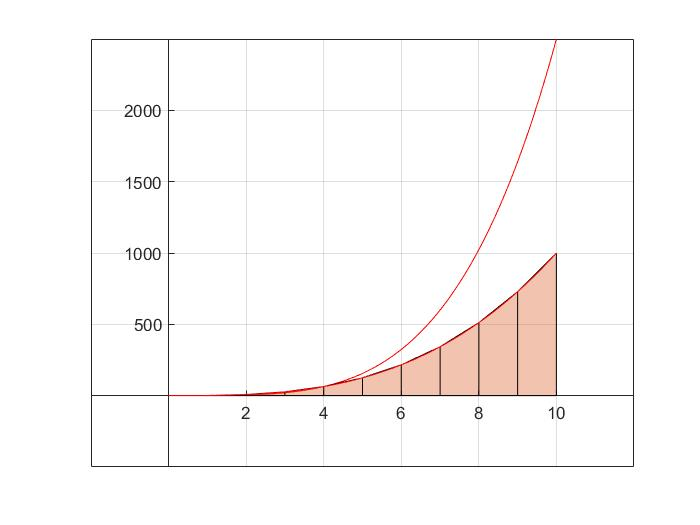
\includegraphics[width=8.2cm]{pic27codeIntegral.jpg}
    \caption{ روش ذوزنقه اي مرکب $y=x^3$ }
    \label{fig:انتگرال خط}
\end{figure}

\begin{figure}[!h]
    \centering
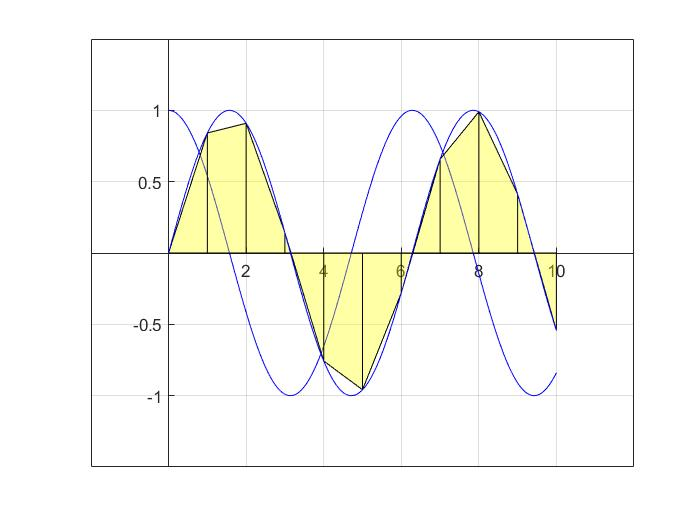
\includegraphics[width=8.2cm]{pic28codeIntegral.jpg}
    \caption{ روش ذوزنقه اي مرکب $y=sin(x)$ }
    \label{fig:انتگرال خط}
\end{figure}


\begin{figure}[!h]
    \centering
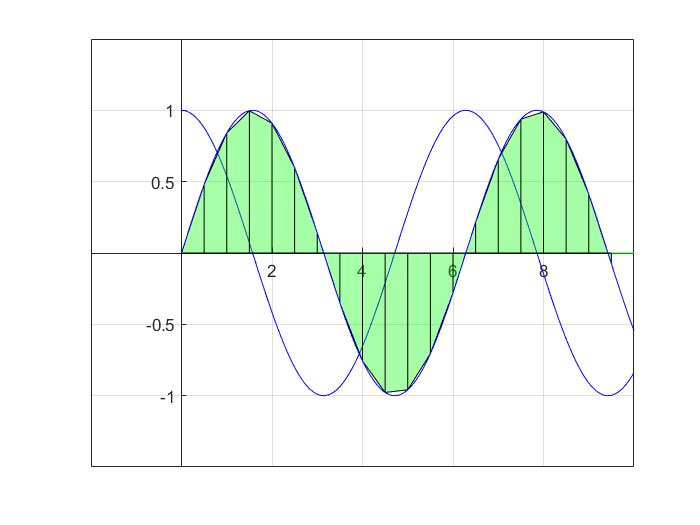
\includegraphics[width=8.2cm]{pic29codeIntegral.jpg}
    \caption{ روش ذوزنقه اي مرکب $y=sin(x)$ }
    \label{fig:انتگرال خط}
\end{figure}

\begin{figure}[!h]
    \centering
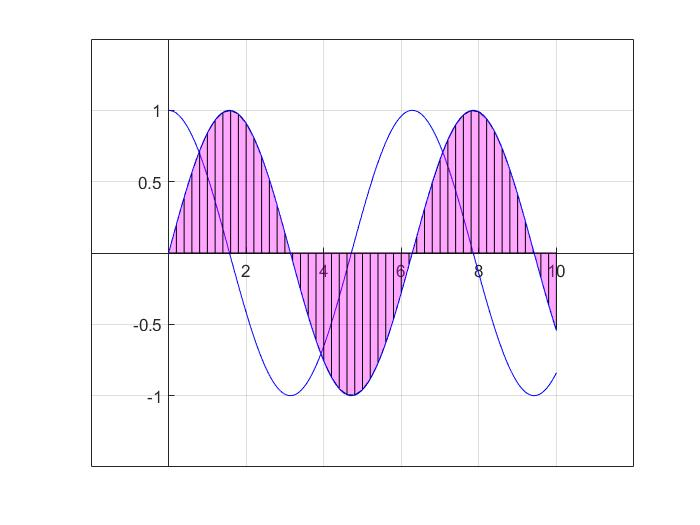
\includegraphics[width=8.2cm]{pic31codeIntegral.jpg}
    \caption{ روش ذوزنقه اي مرکب $y=sin(x)$ }
    \label{fig:انتگرال خط}
\end{figure}

\begin{figure}[!h]
    \centering
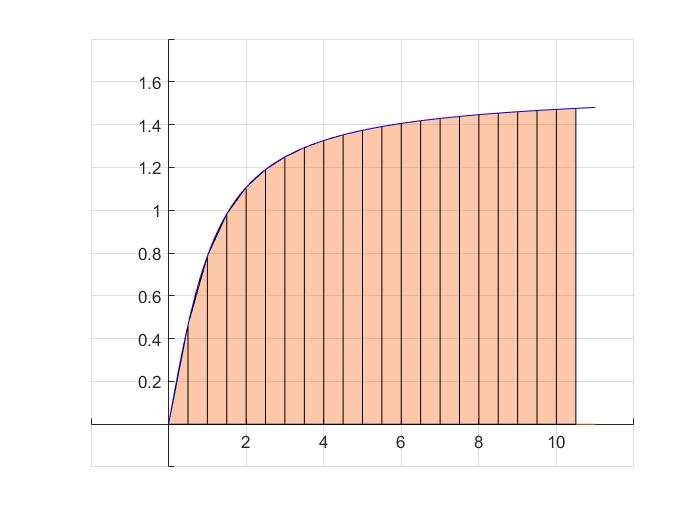
\includegraphics[width=8.2cm]{pic45codeIntegral.jpg}
    \caption{ روش ذوزنقه اي مرکب $y=arctan(x)$ }
    \label{fig:انتگرال خط}
\end{figure}

\begin{figure}[!h]
    \centering
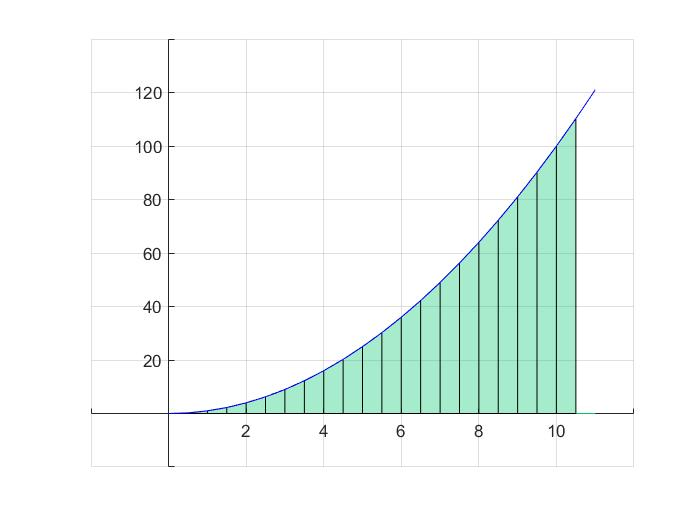
\includegraphics[width=8.2cm]{pic46codeIntegral.jpg}
    \caption{ روش ذوزنقه اي مرکب $y=x^2$ }
    \label{fig:انتگرال خط}
\end{figure}

\newpage
ثابت می شود $c$
وجود دارد به طوری که 


\begin{align*}
    \int_{a}^{b} f(x)dx - T_{n}(f) =\dfrac {-(b-a)}{2} h^2 f''(c)
\end{align*}

\pagebreak
\bibliographystyle{unsrt-fa}
\bibliography{lib}



\end{document}
